\documentclass[preview]{standalone}
\usepackage[table,dvipsnames]{xcolor}
\colorlet{colorCondition}{RedOrange}
\colorlet{colorAttribute}{PineGreen!75!green!85!black}
\colorlet{colorSync}{Blue}
\colorlet{colorTransition}{blue}
\usepackage{tikz}
\usetikzlibrary{arrows, automata, positioning}
\tikzset{initial text =\(\)}
\begin{document}
\begin{figure}
\centering
\scalebox{.75}{
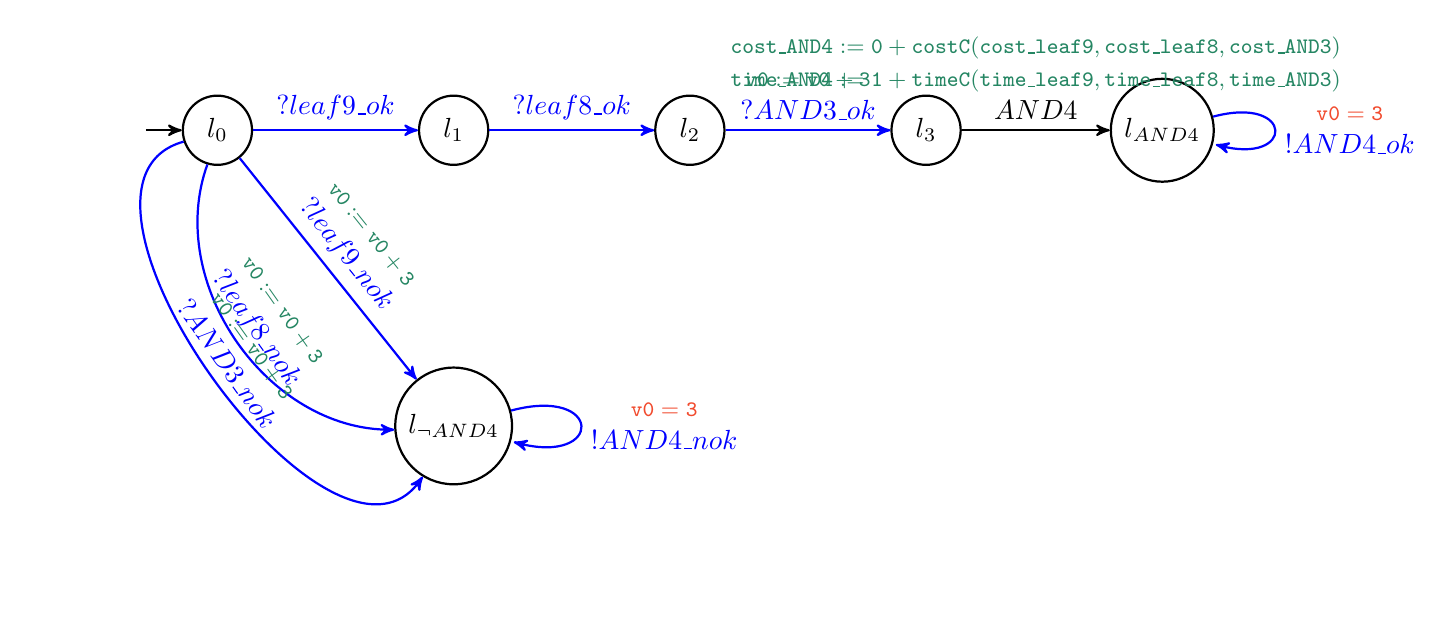
\begin{tikzpicture}[>=stealth', thick, node distance=3cm, every node/.style={sloped}]
\node[state, initial] (q0) {$l_{0}$};
\node[state, right of =q0] (q1) {$l_{1}$};
\node[state, right of =q1] (q2) {$l_{2}$};
\node[state, right of =q2] (q3) {$l_{3}$};
\node[state, right of =q3] (q5) {$l_{AND4}$};
\node[state, right of =q0, below=3cm] (q4) {$l_{\neg AND4}$};
\draw [->, colorTransition] (q0) edge [, bend right=0,above, align=center, ] node []{\textcolor{colorSync}{$?leaf9\_ok$}} (q1);
\draw [->, colorTransition] (q0) edge [, bend right=0,above, align=center, ] node []{\footnotesize{\textcolor{colorAttribute}{$\mathtt{v0 : = v0+3}$}}\\\textcolor{colorSync}{$?leaf9\_nok$}} (q4);
\draw [->, colorTransition] (q0) edge [, bend right=55,above, align=center, ] node []{\footnotesize{\textcolor{colorAttribute}{$\mathtt{v0 : = v0+3}$}}\\\textcolor{colorSync}{$?leaf8\_nok$}} (q4);
\draw [->, colorTransition] (q0) edge [, bend right=110,above, align=center, ] node []{\footnotesize{\textcolor{colorAttribute}{$\mathtt{v0 : = v0+3}$}}\\\textcolor{colorSync}{$?AND3\_nok$}} (q4);
\draw [->, colorTransition] (q1) edge [, bend right=0,above, align=center, ] node []{\textcolor{colorSync}{$?leaf8\_ok$}} (q2);
\draw [->, colorTransition] (q2) edge [, bend right=0,above, align=center, ] node []{\footnotesize{\textcolor{colorAttribute}{$\mathtt{v0 : = v0+3}$}}\\\textcolor{colorSync}{$?AND3\_ok$}} (q3);
\draw [->, black] (q3) edge [, bend right=0,above, align=center, ] node []{\footnotesize{\textcolor{colorAttribute}{$\mathtt{cost\_AND4 : = 0+costC(cost\_leaf9,cost\_leaf8,cost\_AND3)}$}}\\\footnotesize{\textcolor{colorAttribute}{$\mathtt{time\_AND4 : = 1+timeC(time\_leaf9,time\_leaf8,time\_AND3)}$}}\\\textcolor{black}{$AND4$}} (q5);
\draw [->, colorTransition] (q5) edge [loop right, above, align=center, ] node [rotate=90, anchor=west]{\footnotesize{\textcolor{colorCondition}{$\mathtt{v0=3}$}}\\\textcolor{colorSync}{$!AND4\_ok$}} (q5);
\draw [->, colorTransition] (q4) edge [loop right, above, align=center, ] node [rotate=90, anchor=west]{\footnotesize{\textcolor{colorCondition}{$\mathtt{v0=3}$}}\\\textcolor{colorSync}{$!AND4\_nok$}} (q4);
\end{tikzpicture}
}
\caption{EAMAS model for the ADTree node AND4} \label{fig:AND4}
\end{figure}

\begin{figure}
\centering
\scalebox{.75}{
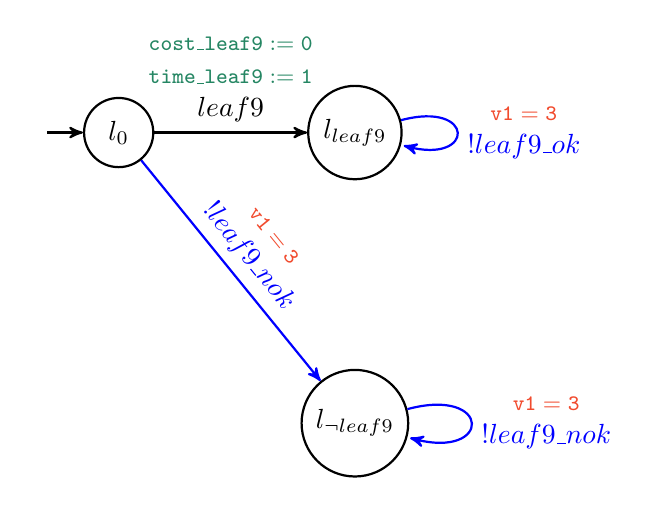
\begin{tikzpicture}[>=stealth', thick, node distance=3cm, every node/.style={sloped}]
\node[state, initial] (q6) {$l_{0}$};
\node[state, right of =q6] (q7) {$l_{leaf9}$};
\node[state, right of =q6, below=3cm] (q8) {$l_{\neg leaf9}$};
\draw [->, black] (q6) edge [, bend right=0,above, align=center, ] node []{\footnotesize{\textcolor{colorAttribute}{$\mathtt{cost\_leaf9 : = 0}$}}\\\footnotesize{\textcolor{colorAttribute}{$\mathtt{time\_leaf9 : = 1}$}}\\\textcolor{black}{$leaf9$}} (q7);
\draw [->, colorTransition] (q6) edge [, bend right=0,above, align=center, ] node []{\footnotesize{\textcolor{colorCondition}{$\mathtt{v1=3}$}}\\\textcolor{colorSync}{$!leaf9\_nok$}} (q8);
\draw [->, colorTransition] (q7) edge [loop right, above, align=center, ] node [rotate=90, anchor=west]{\footnotesize{\textcolor{colorCondition}{$\mathtt{v1=3}$}}\\\textcolor{colorSync}{$!leaf9\_ok$}} (q7);
\draw [->, colorTransition] (q8) edge [loop right, above, align=center, ] node [rotate=90, anchor=west]{\footnotesize{\textcolor{colorCondition}{$\mathtt{v1=3}$}}\\\textcolor{colorSync}{$!leaf9\_nok$}} (q8);
\end{tikzpicture}
}
\caption{EAMAS model for the ADTree node leaf9} \label{fig:leaf9}
\end{figure}

\begin{figure}
\centering
\scalebox{.75}{
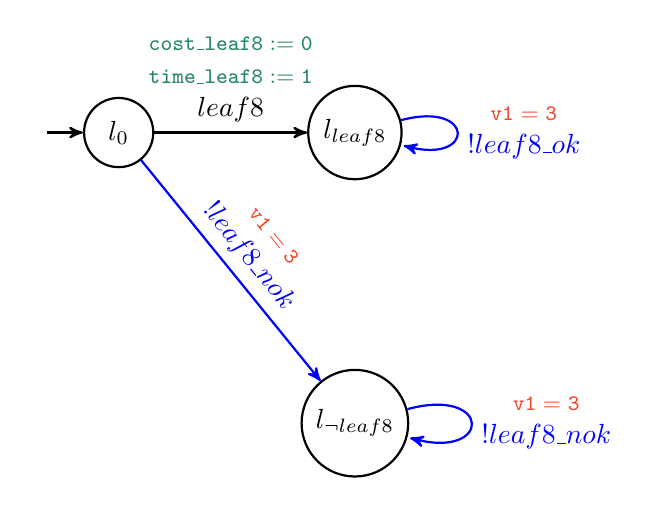
\begin{tikzpicture}[>=stealth', thick, node distance=3cm, every node/.style={sloped}]
\node[state, initial] (q9) {$l_{0}$};
\node[state, right of =q9] (q10) {$l_{leaf8}$};
\node[state, right of =q9, below=3cm] (q11) {$l_{\neg leaf8}$};
\draw [->, black] (q9) edge [, bend right=0,above, align=center, ] node []{\footnotesize{\textcolor{colorAttribute}{$\mathtt{cost\_leaf8 : = 0}$}}\\\footnotesize{\textcolor{colorAttribute}{$\mathtt{time\_leaf8 : = 1}$}}\\\textcolor{black}{$leaf8$}} (q10);
\draw [->, colorTransition] (q9) edge [, bend right=0,above, align=center, ] node []{\footnotesize{\textcolor{colorCondition}{$\mathtt{v1=3}$}}\\\textcolor{colorSync}{$!leaf8\_nok$}} (q11);
\draw [->, colorTransition] (q10) edge [loop right, above, align=center, ] node [rotate=90, anchor=west]{\footnotesize{\textcolor{colorCondition}{$\mathtt{v1=3}$}}\\\textcolor{colorSync}{$!leaf8\_ok$}} (q10);
\draw [->, colorTransition] (q11) edge [loop right, above, align=center, ] node [rotate=90, anchor=west]{\footnotesize{\textcolor{colorCondition}{$\mathtt{v1=3}$}}\\\textcolor{colorSync}{$!leaf8\_nok$}} (q11);
\end{tikzpicture}
}
\caption{EAMAS model for the ADTree node leaf8} \label{fig:leaf8}
\end{figure}

\begin{figure}
\centering
\scalebox{.75}{
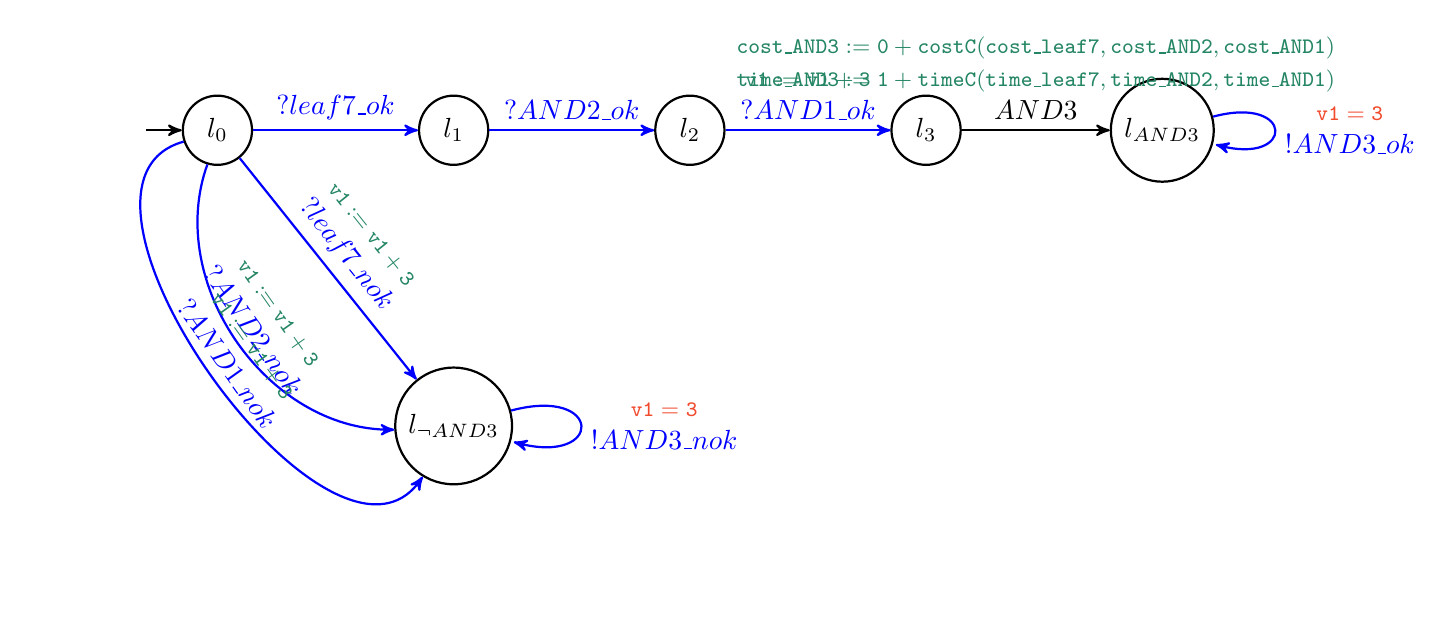
\begin{tikzpicture}[>=stealth', thick, node distance=3cm, every node/.style={sloped}]
\node[state, initial] (q12) {$l_{0}$};
\node[state, right of =q12] (q13) {$l_{1}$};
\node[state, right of =q13] (q14) {$l_{2}$};
\node[state, right of =q14] (q15) {$l_{3}$};
\node[state, right of =q15] (q17) {$l_{AND3}$};
\node[state, right of =q12, below=3cm] (q16) {$l_{\neg AND3}$};
\draw [->, colorTransition] (q12) edge [, bend right=0,above, align=center, ] node []{\textcolor{colorSync}{$?leaf7\_ok$}} (q13);
\draw [->, colorTransition] (q12) edge [, bend right=0,above, align=center, ] node []{\footnotesize{\textcolor{colorAttribute}{$\mathtt{v1 : = v1+3}$}}\\\textcolor{colorSync}{$?leaf7\_nok$}} (q16);
\draw [->, colorTransition] (q12) edge [, bend right=55,above, align=center, ] node []{\footnotesize{\textcolor{colorAttribute}{$\mathtt{v1 : = v1+3}$}}\\\textcolor{colorSync}{$?AND2\_nok$}} (q16);
\draw [->, colorTransition] (q12) edge [, bend right=110,above, align=center, ] node []{\footnotesize{\textcolor{colorAttribute}{$\mathtt{v1 : = v1+3}$}}\\\textcolor{colorSync}{$?AND1\_nok$}} (q16);
\draw [->, colorTransition] (q13) edge [, bend right=0,above, align=center, ] node []{\textcolor{colorSync}{$?AND2\_ok$}} (q14);
\draw [->, colorTransition] (q14) edge [, bend right=0,above, align=center, ] node []{\footnotesize{\textcolor{colorAttribute}{$\mathtt{v1 : = v1+3}$}}\\\textcolor{colorSync}{$?AND1\_ok$}} (q15);
\draw [->, black] (q15) edge [, bend right=0,above, align=center, ] node []{\footnotesize{\textcolor{colorAttribute}{$\mathtt{cost\_AND3 : = 0+costC(cost\_leaf7,cost\_AND2,cost\_AND1)}$}}\\\footnotesize{\textcolor{colorAttribute}{$\mathtt{time\_AND3 : = 1+timeC(time\_leaf7,time\_AND2,time\_AND1)}$}}\\\textcolor{black}{$AND3$}} (q17);
\draw [->, colorTransition] (q17) edge [loop right, above, align=center, ] node [rotate=90, anchor=west]{\footnotesize{\textcolor{colorCondition}{$\mathtt{v1=3}$}}\\\textcolor{colorSync}{$!AND3\_ok$}} (q17);
\draw [->, colorTransition] (q16) edge [loop right, above, align=center, ] node [rotate=90, anchor=west]{\footnotesize{\textcolor{colorCondition}{$\mathtt{v1=3}$}}\\\textcolor{colorSync}{$!AND3\_nok$}} (q16);
\end{tikzpicture}
}
\caption{EAMAS model for the ADTree node AND3} \label{fig:AND3}
\end{figure}

\begin{figure}
\centering
\scalebox{.75}{
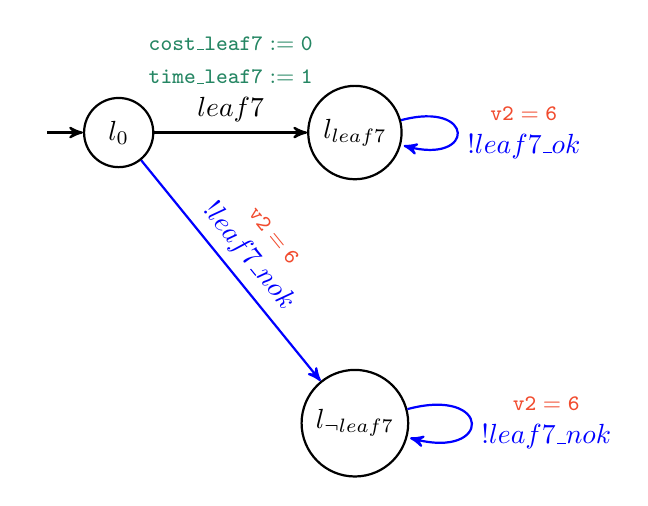
\begin{tikzpicture}[>=stealth', thick, node distance=3cm, every node/.style={sloped}]
\node[state, initial] (q18) {$l_{0}$};
\node[state, right of =q18] (q19) {$l_{leaf7}$};
\node[state, right of =q18, below=3cm] (q20) {$l_{\neg leaf7}$};
\draw [->, black] (q18) edge [, bend right=0,above, align=center, ] node []{\footnotesize{\textcolor{colorAttribute}{$\mathtt{cost\_leaf7 : = 0}$}}\\\footnotesize{\textcolor{colorAttribute}{$\mathtt{time\_leaf7 : = 1}$}}\\\textcolor{black}{$leaf7$}} (q19);
\draw [->, colorTransition] (q18) edge [, bend right=0,above, align=center, ] node []{\footnotesize{\textcolor{colorCondition}{$\mathtt{v2=6}$}}\\\textcolor{colorSync}{$!leaf7\_nok$}} (q20);
\draw [->, colorTransition] (q19) edge [loop right, above, align=center, ] node [rotate=90, anchor=west]{\footnotesize{\textcolor{colorCondition}{$\mathtt{v2=6}$}}\\\textcolor{colorSync}{$!leaf7\_ok$}} (q19);
\draw [->, colorTransition] (q20) edge [loop right, above, align=center, ] node [rotate=90, anchor=west]{\footnotesize{\textcolor{colorCondition}{$\mathtt{v2=6}$}}\\\textcolor{colorSync}{$!leaf7\_nok$}} (q20);
\end{tikzpicture}
}
\caption{EAMAS model for the ADTree node leaf7} \label{fig:leaf7}
\end{figure}

\begin{figure}
\centering
\scalebox{.75}{
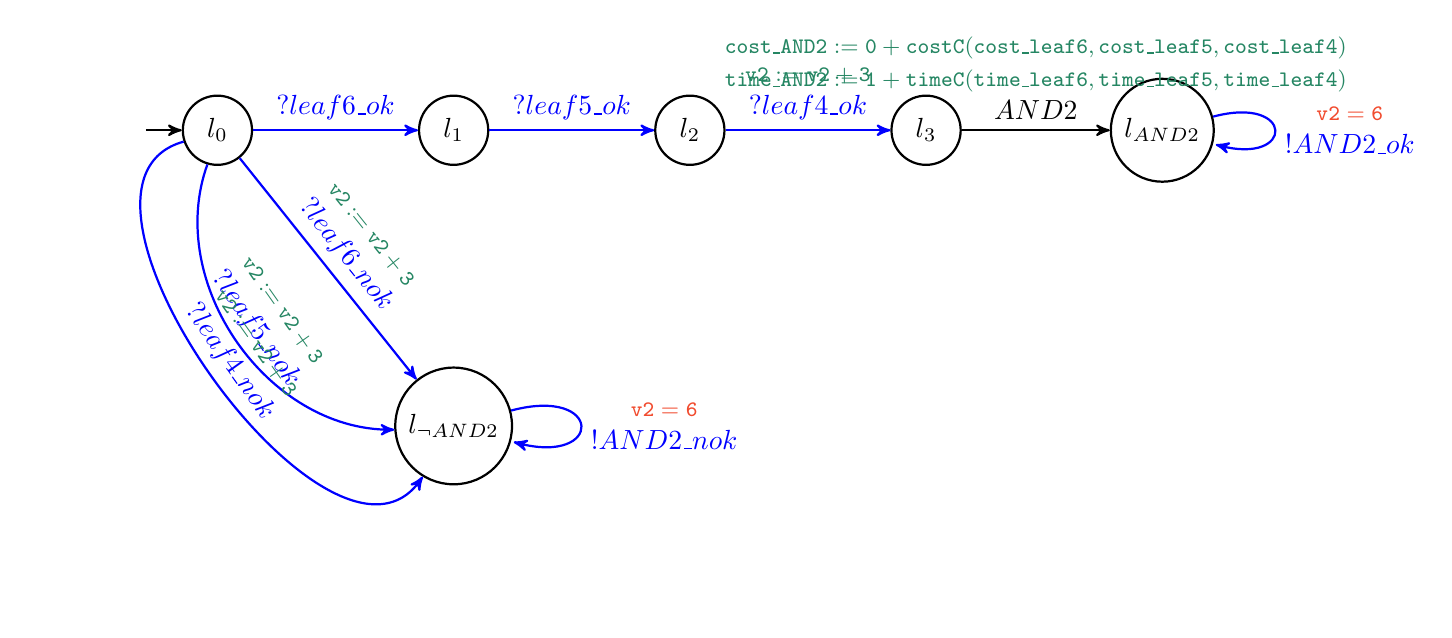
\begin{tikzpicture}[>=stealth', thick, node distance=3cm, every node/.style={sloped}]
\node[state, initial] (q21) {$l_{0}$};
\node[state, right of =q21] (q22) {$l_{1}$};
\node[state, right of =q22] (q23) {$l_{2}$};
\node[state, right of =q23] (q24) {$l_{3}$};
\node[state, right of =q24] (q26) {$l_{AND2}$};
\node[state, right of =q21, below=3cm] (q25) {$l_{\neg AND2}$};
\draw [->, colorTransition] (q21) edge [, bend right=0,above, align=center, ] node []{\textcolor{colorSync}{$?leaf6\_ok$}} (q22);
\draw [->, colorTransition] (q21) edge [, bend right=0,above, align=center, ] node []{\footnotesize{\textcolor{colorAttribute}{$\mathtt{v2 : = v2+3}$}}\\\textcolor{colorSync}{$?leaf6\_nok$}} (q25);
\draw [->, colorTransition] (q21) edge [, bend right=55,above, align=center, ] node []{\footnotesize{\textcolor{colorAttribute}{$\mathtt{v2 : = v2+3}$}}\\\textcolor{colorSync}{$?leaf5\_nok$}} (q25);
\draw [->, colorTransition] (q21) edge [, bend right=110,above, align=center, ] node []{\footnotesize{\textcolor{colorAttribute}{$\mathtt{v2 : = v2+3}$}}\\\textcolor{colorSync}{$?leaf4\_nok$}} (q25);
\draw [->, colorTransition] (q22) edge [, bend right=0,above, align=center, ] node []{\textcolor{colorSync}{$?leaf5\_ok$}} (q23);
\draw [->, colorTransition] (q23) edge [, bend right=0,above, align=center, ] node []{\footnotesize{\textcolor{colorAttribute}{$\mathtt{v2 : = v2+3}$}}\\\textcolor{colorSync}{$?leaf4\_ok$}} (q24);
\draw [->, black] (q24) edge [, bend right=0,above, align=center, ] node []{\footnotesize{\textcolor{colorAttribute}{$\mathtt{cost\_AND2 : = 0+costC(cost\_leaf6,cost\_leaf5,cost\_leaf4)}$}}\\\footnotesize{\textcolor{colorAttribute}{$\mathtt{time\_AND2 : = 1+timeC(time\_leaf6,time\_leaf5,time\_leaf4)}$}}\\\textcolor{black}{$AND2$}} (q26);
\draw [->, colorTransition] (q26) edge [loop right, above, align=center, ] node [rotate=90, anchor=west]{\footnotesize{\textcolor{colorCondition}{$\mathtt{v2=6}$}}\\\textcolor{colorSync}{$!AND2\_ok$}} (q26);
\draw [->, colorTransition] (q25) edge [loop right, above, align=center, ] node [rotate=90, anchor=west]{\footnotesize{\textcolor{colorCondition}{$\mathtt{v2=6}$}}\\\textcolor{colorSync}{$!AND2\_nok$}} (q25);
\end{tikzpicture}
}
\caption{EAMAS model for the ADTree node AND2} \label{fig:AND2}
\end{figure}

\begin{figure}
\centering
\scalebox{.75}{
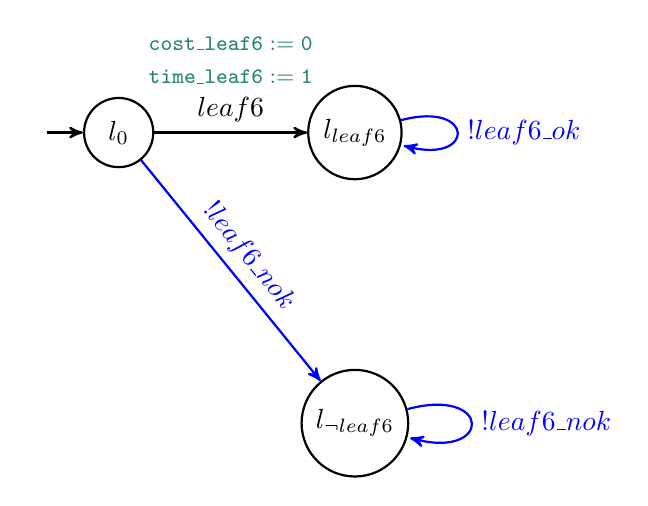
\begin{tikzpicture}[>=stealth', thick, node distance=3cm, every node/.style={sloped}]
\node[state, initial] (q27) {$l_{0}$};
\node[state, right of =q27] (q28) {$l_{leaf6}$};
\node[state, right of =q27, below=3cm] (q29) {$l_{\neg leaf6}$};
\draw [->, black] (q27) edge [, bend right=0,above, align=center, ] node []{\footnotesize{\textcolor{colorAttribute}{$\mathtt{cost\_leaf6 : = 0}$}}\\\footnotesize{\textcolor{colorAttribute}{$\mathtt{time\_leaf6 : = 1}$}}\\\textcolor{black}{$leaf6$}} (q28);
\draw [->, colorTransition] (q27) edge [, bend right=0,above, align=center, ] node []{\textcolor{colorSync}{$!leaf6\_nok$}} (q29);
\draw [->, colorTransition] (q28) edge [loop right, above, align=center, ] node [rotate=90, anchor=west]{\textcolor{colorSync}{$!leaf6\_ok$}} (q28);
\draw [->, colorTransition] (q29) edge [loop right, above, align=center, ] node [rotate=90, anchor=west]{\textcolor{colorSync}{$!leaf6\_nok$}} (q29);
\end{tikzpicture}
}
\caption{EAMAS model for the ADTree node leaf6} \label{fig:leaf6}
\end{figure}

\begin{figure}
\centering
\scalebox{.75}{
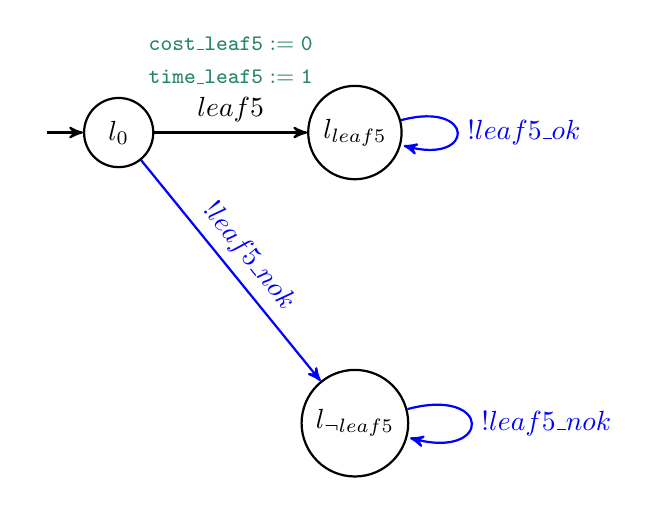
\begin{tikzpicture}[>=stealth', thick, node distance=3cm, every node/.style={sloped}]
\node[state, initial] (q30) {$l_{0}$};
\node[state, right of =q30] (q31) {$l_{leaf5}$};
\node[state, right of =q30, below=3cm] (q32) {$l_{\neg leaf5}$};
\draw [->, black] (q30) edge [, bend right=0,above, align=center, ] node []{\footnotesize{\textcolor{colorAttribute}{$\mathtt{cost\_leaf5 : = 0}$}}\\\footnotesize{\textcolor{colorAttribute}{$\mathtt{time\_leaf5 : = 1}$}}\\\textcolor{black}{$leaf5$}} (q31);
\draw [->, colorTransition] (q30) edge [, bend right=0,above, align=center, ] node []{\textcolor{colorSync}{$!leaf5\_nok$}} (q32);
\draw [->, colorTransition] (q31) edge [loop right, above, align=center, ] node [rotate=90, anchor=west]{\textcolor{colorSync}{$!leaf5\_ok$}} (q31);
\draw [->, colorTransition] (q32) edge [loop right, above, align=center, ] node [rotate=90, anchor=west]{\textcolor{colorSync}{$!leaf5\_nok$}} (q32);
\end{tikzpicture}
}
\caption{EAMAS model for the ADTree node leaf5} \label{fig:leaf5}
\end{figure}

\begin{figure}
\centering
\scalebox{.75}{
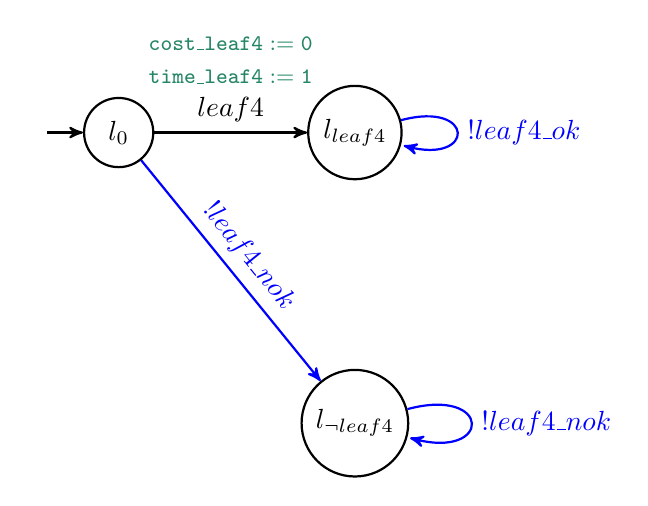
\begin{tikzpicture}[>=stealth', thick, node distance=3cm, every node/.style={sloped}]
\node[state, initial] (q33) {$l_{0}$};
\node[state, right of =q33] (q34) {$l_{leaf4}$};
\node[state, right of =q33, below=3cm] (q35) {$l_{\neg leaf4}$};
\draw [->, black] (q33) edge [, bend right=0,above, align=center, ] node []{\footnotesize{\textcolor{colorAttribute}{$\mathtt{cost\_leaf4 : = 0}$}}\\\footnotesize{\textcolor{colorAttribute}{$\mathtt{time\_leaf4 : = 1}$}}\\\textcolor{black}{$leaf4$}} (q34);
\draw [->, colorTransition] (q33) edge [, bend right=0,above, align=center, ] node []{\textcolor{colorSync}{$!leaf4\_nok$}} (q35);
\draw [->, colorTransition] (q34) edge [loop right, above, align=center, ] node [rotate=90, anchor=west]{\textcolor{colorSync}{$!leaf4\_ok$}} (q34);
\draw [->, colorTransition] (q35) edge [loop right, above, align=center, ] node [rotate=90, anchor=west]{\textcolor{colorSync}{$!leaf4\_nok$}} (q35);
\end{tikzpicture}
}
\caption{EAMAS model for the ADTree node leaf4} \label{fig:leaf4}
\end{figure}

\begin{figure}
\centering
\scalebox{.75}{
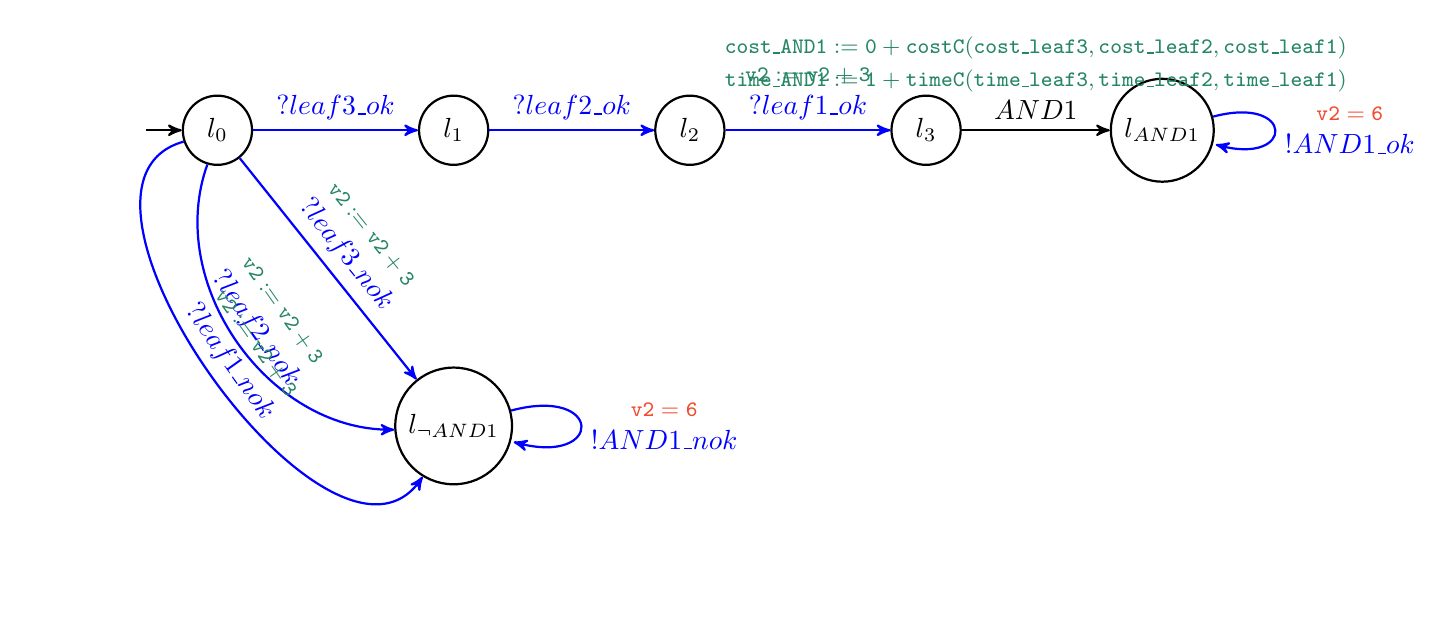
\begin{tikzpicture}[>=stealth', thick, node distance=3cm, every node/.style={sloped}]
\node[state, initial] (q36) {$l_{0}$};
\node[state, right of =q36] (q37) {$l_{1}$};
\node[state, right of =q37] (q38) {$l_{2}$};
\node[state, right of =q38] (q39) {$l_{3}$};
\node[state, right of =q39] (q41) {$l_{AND1}$};
\node[state, right of =q36, below=3cm] (q40) {$l_{\neg AND1}$};
\draw [->, colorTransition] (q36) edge [, bend right=0,above, align=center, ] node []{\textcolor{colorSync}{$?leaf3\_ok$}} (q37);
\draw [->, colorTransition] (q36) edge [, bend right=0,above, align=center, ] node []{\footnotesize{\textcolor{colorAttribute}{$\mathtt{v2 : = v2+3}$}}\\\textcolor{colorSync}{$?leaf3\_nok$}} (q40);
\draw [->, colorTransition] (q36) edge [, bend right=55,above, align=center, ] node []{\footnotesize{\textcolor{colorAttribute}{$\mathtt{v2 : = v2+3}$}}\\\textcolor{colorSync}{$?leaf2\_nok$}} (q40);
\draw [->, colorTransition] (q36) edge [, bend right=110,above, align=center, ] node []{\footnotesize{\textcolor{colorAttribute}{$\mathtt{v2 : = v2+3}$}}\\\textcolor{colorSync}{$?leaf1\_nok$}} (q40);
\draw [->, colorTransition] (q37) edge [, bend right=0,above, align=center, ] node []{\textcolor{colorSync}{$?leaf2\_ok$}} (q38);
\draw [->, colorTransition] (q38) edge [, bend right=0,above, align=center, ] node []{\footnotesize{\textcolor{colorAttribute}{$\mathtt{v2 : = v2+3}$}}\\\textcolor{colorSync}{$?leaf1\_ok$}} (q39);
\draw [->, black] (q39) edge [, bend right=0,above, align=center, ] node []{\footnotesize{\textcolor{colorAttribute}{$\mathtt{cost\_AND1 : = 0+costC(cost\_leaf3,cost\_leaf2,cost\_leaf1)}$}}\\\footnotesize{\textcolor{colorAttribute}{$\mathtt{time\_AND1 : = 1+timeC(time\_leaf3,time\_leaf2,time\_leaf1)}$}}\\\textcolor{black}{$AND1$}} (q41);
\draw [->, colorTransition] (q41) edge [loop right, above, align=center, ] node [rotate=90, anchor=west]{\footnotesize{\textcolor{colorCondition}{$\mathtt{v2=6}$}}\\\textcolor{colorSync}{$!AND1\_ok$}} (q41);
\draw [->, colorTransition] (q40) edge [loop right, above, align=center, ] node [rotate=90, anchor=west]{\footnotesize{\textcolor{colorCondition}{$\mathtt{v2=6}$}}\\\textcolor{colorSync}{$!AND1\_nok$}} (q40);
\end{tikzpicture}
}
\caption{EAMAS model for the ADTree node AND1} \label{fig:AND1}
\end{figure}

\begin{figure}
\centering
\scalebox{.75}{
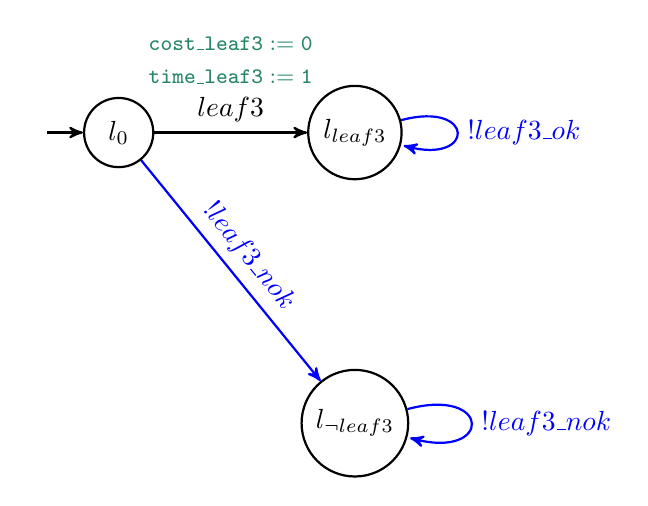
\begin{tikzpicture}[>=stealth', thick, node distance=3cm, every node/.style={sloped}]
\node[state, initial] (q42) {$l_{0}$};
\node[state, right of =q42] (q43) {$l_{leaf3}$};
\node[state, right of =q42, below=3cm] (q44) {$l_{\neg leaf3}$};
\draw [->, black] (q42) edge [, bend right=0,above, align=center, ] node []{\footnotesize{\textcolor{colorAttribute}{$\mathtt{cost\_leaf3 : = 0}$}}\\\footnotesize{\textcolor{colorAttribute}{$\mathtt{time\_leaf3 : = 1}$}}\\\textcolor{black}{$leaf3$}} (q43);
\draw [->, colorTransition] (q42) edge [, bend right=0,above, align=center, ] node []{\textcolor{colorSync}{$!leaf3\_nok$}} (q44);
\draw [->, colorTransition] (q43) edge [loop right, above, align=center, ] node [rotate=90, anchor=west]{\textcolor{colorSync}{$!leaf3\_ok$}} (q43);
\draw [->, colorTransition] (q44) edge [loop right, above, align=center, ] node [rotate=90, anchor=west]{\textcolor{colorSync}{$!leaf3\_nok$}} (q44);
\end{tikzpicture}
}
\caption{EAMAS model for the ADTree node leaf3} \label{fig:leaf3}
\end{figure}

\begin{figure}
\centering
\scalebox{.75}{
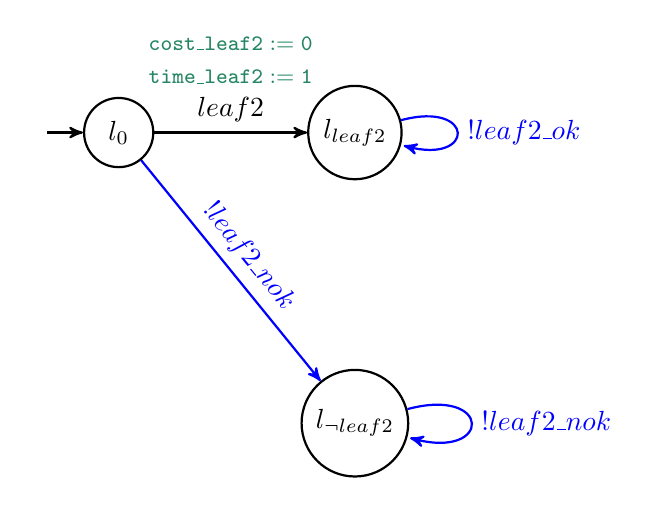
\begin{tikzpicture}[>=stealth', thick, node distance=3cm, every node/.style={sloped}]
\node[state, initial] (q45) {$l_{0}$};
\node[state, right of =q45] (q46) {$l_{leaf2}$};
\node[state, right of =q45, below=3cm] (q47) {$l_{\neg leaf2}$};
\draw [->, black] (q45) edge [, bend right=0,above, align=center, ] node []{\footnotesize{\textcolor{colorAttribute}{$\mathtt{cost\_leaf2 : = 0}$}}\\\footnotesize{\textcolor{colorAttribute}{$\mathtt{time\_leaf2 : = 1}$}}\\\textcolor{black}{$leaf2$}} (q46);
\draw [->, colorTransition] (q45) edge [, bend right=0,above, align=center, ] node []{\textcolor{colorSync}{$!leaf2\_nok$}} (q47);
\draw [->, colorTransition] (q46) edge [loop right, above, align=center, ] node [rotate=90, anchor=west]{\textcolor{colorSync}{$!leaf2\_ok$}} (q46);
\draw [->, colorTransition] (q47) edge [loop right, above, align=center, ] node [rotate=90, anchor=west]{\textcolor{colorSync}{$!leaf2\_nok$}} (q47);
\end{tikzpicture}
}
\caption{EAMAS model for the ADTree node leaf2} \label{fig:leaf2}
\end{figure}

\begin{figure}
\centering
\scalebox{.75}{
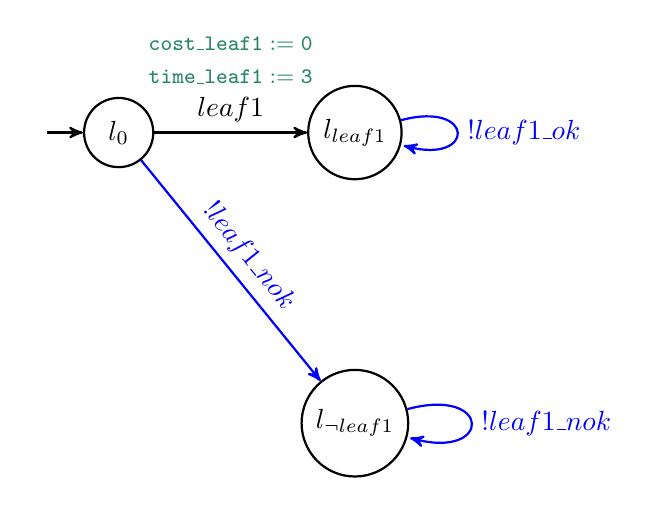
\begin{tikzpicture}[>=stealth', thick, node distance=3cm, every node/.style={sloped}]
\node[state, initial] (q48) {$l_{0}$};
\node[state, right of =q48] (q49) {$l_{leaf1}$};
\node[state, right of =q48, below=3cm] (q50) {$l_{\neg leaf1}$};
\draw [->, black] (q48) edge [, bend right=0,above, align=center, ] node []{\footnotesize{\textcolor{colorAttribute}{$\mathtt{cost\_leaf1 : = 0}$}}\\\footnotesize{\textcolor{colorAttribute}{$\mathtt{time\_leaf1 : = 3}$}}\\\textcolor{black}{$leaf1$}} (q49);
\draw [->, colorTransition] (q48) edge [, bend right=0,above, align=center, ] node []{\textcolor{colorSync}{$!leaf1\_nok$}} (q50);
\draw [->, colorTransition] (q49) edge [loop right, above, align=center, ] node [rotate=90, anchor=west]{\textcolor{colorSync}{$!leaf1\_ok$}} (q49);
\draw [->, colorTransition] (q50) edge [loop right, above, align=center, ] node [rotate=90, anchor=west]{\textcolor{colorSync}{$!leaf1\_nok$}} (q50);
\end{tikzpicture}
}
\caption{EAMAS model for the ADTree node leaf1} \label{fig:leaf1}
\end{figure}


\end{document}
